%!TEX root = ../document.tex
\chapter{Cross-Site-Scripting}
\label{XSS}
Cross Site Scripting
\section{Erklärung}
blabla bla bla \\ 

\subsection{Angriffsvarianten}
Grundlegend gibt es drei verschiedene Arten von Cross-Site-Scripting Angriffen: \colorbox{altgray}{\lstinline|Reflected XSS, Stored XSS, DOM-Based XSS|}. Um diese möglichst einfach zu erklären, wird im Folgenden der JavaScript Code \colorbox{altgray}{\lstinline|alert("42")|} als Beispiel verwendet. Hierbei kann aber auch jeder andere beliebige JavaScript Code eingeschleust werden. Je nachdem was das Ziel des Angreifers ist, werden bspw. mit \colorbox{altgray}{\lstinline|alert(document.cookie)|}, die gespeicherten Cookies der Webseite auslesen. \\ 
\subsubsection*{Reflected XSS}
\subsubsection*{Stored XSS}
Im Vergleich zum reflektierenden XSS-Angriff unterscheidet sich der Stored XSS (auch persistent/ persistentes XSS) dadurch, dass der Schadcode auf dem Webserver gespeichert wird. Besonders problematisch dabei ist, dass bei jeder Clientanfrage der Schadcode automatisch ausgeliefert und ausgeführt wird. \\ 
\subsubsection*{DOM-Based XSS}
Die dritte Angriffsart von Cross-Site-Scripting bezieht sich ausschließlich auf statische HTML-Seite mit JavaScript Unterstützung lässt dabei den Server außen vor. 
\subsubsection{Gegenmaßnahmen}
... \\ 
Abschließend muss erwähnt werden, dass bestimme Browser wie Google Chrome bereits einen integrierten Cross-Site-Scripting Schutz bieten. Daher ist es zwingend notwendig, dass das nachfolgende Tutorial unter einem Browser ohne XSS-Schutz (z. B. Firefox) durchgeführt wird. 

\section{Ablauf}
Das nachfolgende Kapitel beschreibt den Ablauf der Cross-Site-Scripting Tutorials. Hierzu werden zuerst auf die verschiedenen Übungen des reflektierenden Cross-Site-Scripting vorgestellt. Daraufhin werden jeweils die beiden Aufgaben zu Stored-XSS und DOM-based-XSS beschrieben. Des Weiteren wird zu jeder Beispielaufgabe der Lösungsweg dargelegt. 

\subsection{Reflected Cross-Site-Scripting}

\subsection{Stored Cross-Site-Scripting}
Im Tutorial für die Stored-XSS findet der Einsteiger ein Gästebuch wieder, dem Einträge hinzugefügt werden können. Hierzu sind diese mit einer Datenbank gekoppelt und werden dauerhaft gespeichert. Das Laden der Seite führt dazu, dass die Anwendung sich den Inhalt der Datenbank holt und in eine Tabelle schreibt. Um hier eine Sicherheitslücke zu schaffen werden die Usereingaben nicht überprüft und ungefiltert übermittelt. \\ 
Die Abbildung \ref{fig:stored-xss-aufgabe} zeigt das Gästebuch. Folglich soll der Einsteiger hier ein XSS-Angriff durchführen und die Cookies auslesen. In diesen sind die Credentials mit Username/ Passwort fälschlicherweise gespeichert. \\ 

\begin{figure}[H]
	\centering
	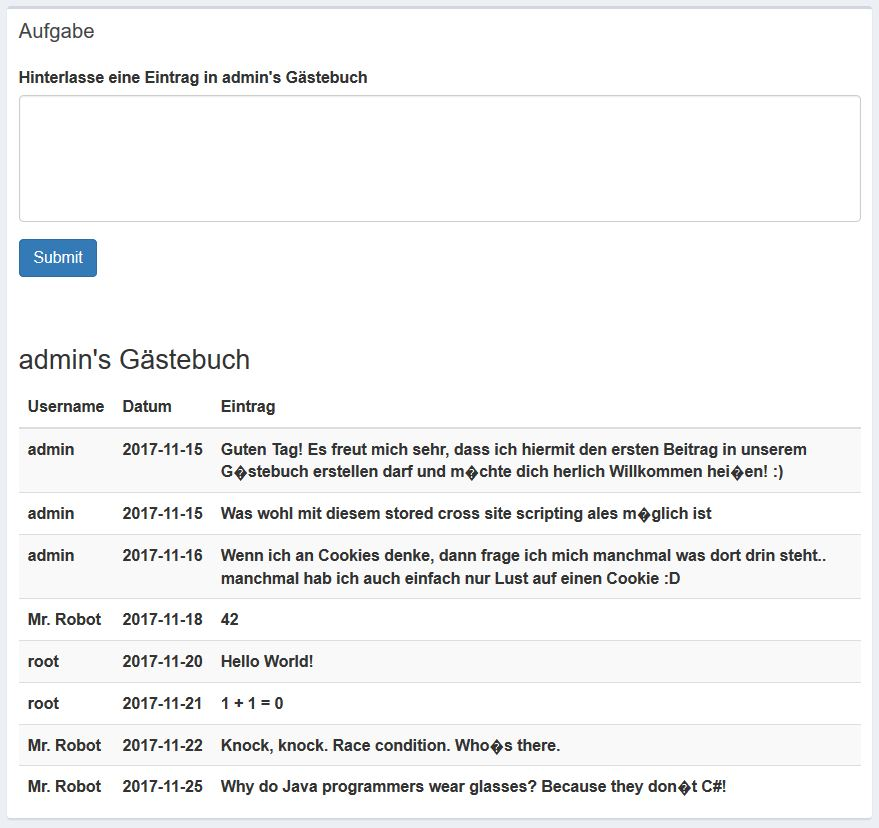
\includegraphics[width=\textwidth]{images/XSS/stored-xss-aufgabe.jpg}
	\caption{Darstellung des theoretischen Hintergrund für Stored-XSS}
	\label{fig:stored-xss-aufgabe}
\end{figure}

Die Lösung für das Tutorial ist es somit, dass der Einsteiger einen Gästebucheintrag verfasst, in dem ein Skript injiziert wird. Ein Beispiel hierfür ist \colorbox{altgray}{\lstinline|<script>alert("Hello World!");</script>|}. Da es für die Lösung der Aufgabe erforderlich ist die Cookies auszulesen, muss der Eintrag die folgende Zeichensequenz enthalten: 
\begin{center} 
\colorbox{altgray}{\lstinline|<script>alert("document.cookie");</script>|} 
\end{center}

Um den Einsteiger optimal auf die Übung vorzubereiten, besitzt dieses Tutorial ein Video mit dem theoretischen Hintergrund für Stored-XSS. Zudem werden dem Einsteiger Tipps an die Hand gegeben um die Aufgabe zu lösen. Abschließend ist zu erwähnen, dass auf dieser Tutorialseite auch die Gegenmaßnahmen dargestellt sind. Die Abbildung \ref{fig:stored-xss-theorie} veranschaulicht das eben Beschriebene. 

\begin{figure}[H]
	\centering
	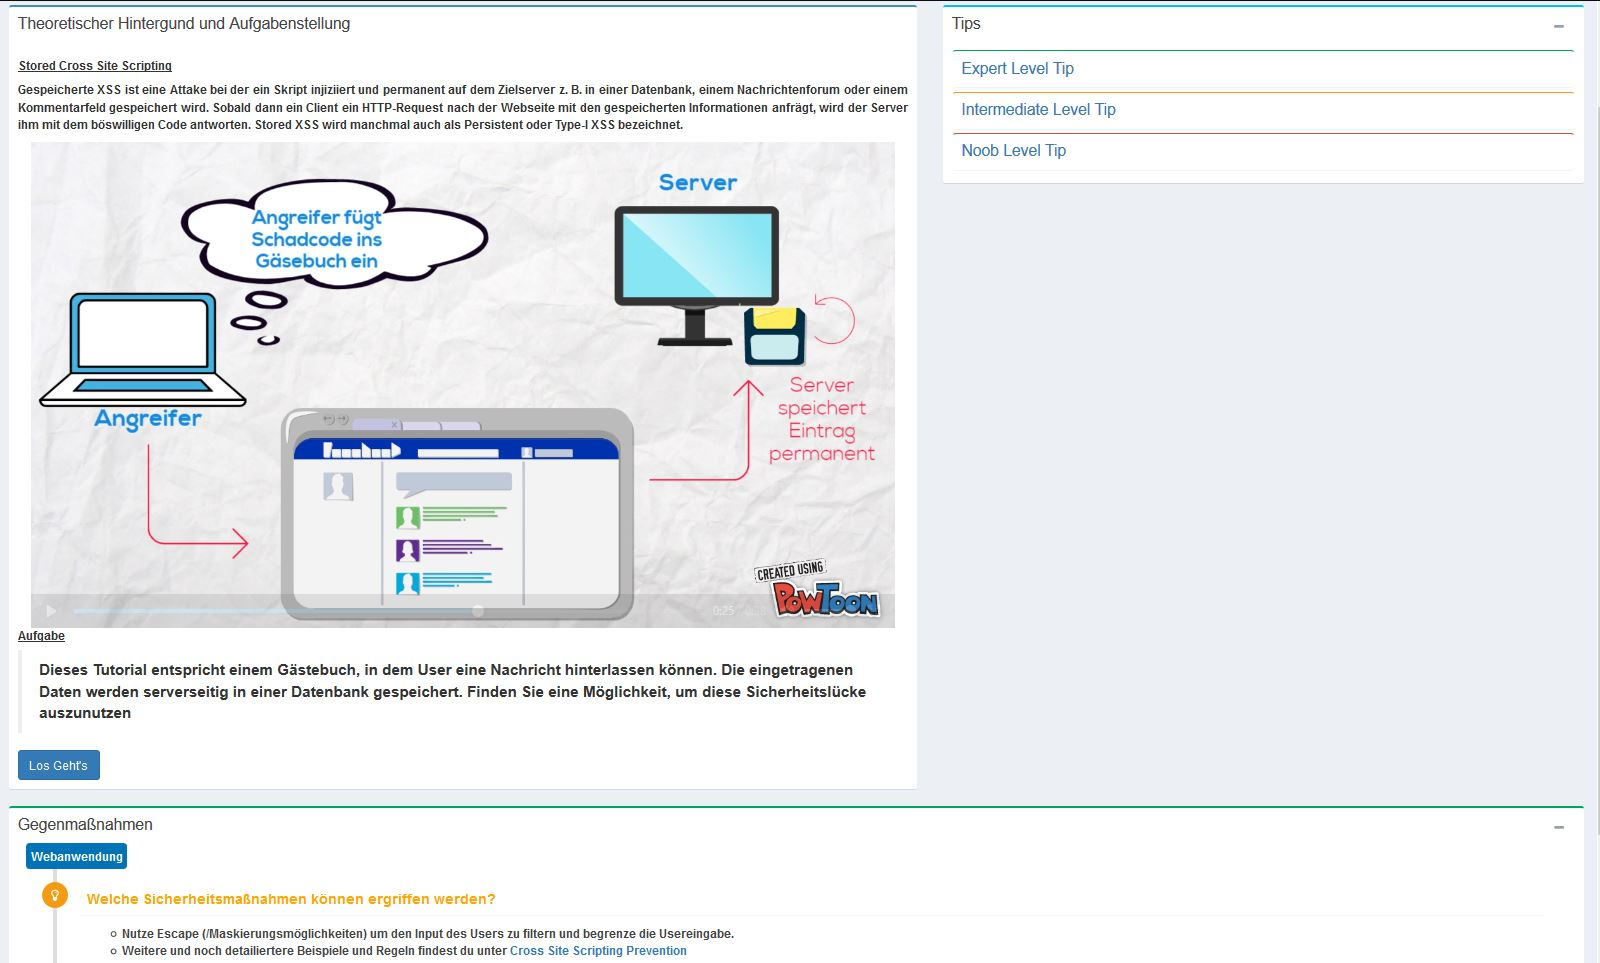
\includegraphics[width=\textwidth]{images/XSS/stored-xss-theorie.jpg}
	\caption{Darstellung des theoretischen Hintergrund für Stored-XSS}
	\label{fig:stored-xss-theorie}
\end{figure}

\subsection{DOM-Based Cross-Site-Scripting}
Das letzte Tutorial in Bezug auf XSS-Angriffe befasst sich mit der Variante des DOM-Based-XSS. \\ 
Hierzu wurde exemplarisch eine Sprachauswahl implementiert, bei der eine Selektierungsmöglichkeit über die URL erzeugt wird. Das folgende Listing \ref{lstlisting:Select-DOM-based} zeigt diesen Anwendungskontext: 
\begin{lstlisting}[caption=Select-Statement\label{lstlisting:Select-DOM-based}]{Name}
<select id="languageList" style='width:500px'>
	<script>
	document.write("<OPTION value=1>" + 				document.location.href.substring(document.location.href.indexOf("default=") + 8) + "</OPTION>");
	</script>
</select>
\end{lstlisting}
Hier wird eine Select-Option über JavaScript erzeugt, indem auf die URL zugegriffen wird. Die Default URL für dieses Tutorial ist \colorbox{altgray}{\lstinline|http://localhost/html/DOMbasedXSS.html?default=german|}. Folglich entspricht eine Auswahlmöglich der Sprache \textit{german}, die restlichen Wahlmöglichkeiten werden über JavaScript inkludiert. Die Abbildung \ref{fig:dom-based-xss-aufgabe} zeigt die Aufgabenstellung. 
\begin{figure}[H]
	\centering
	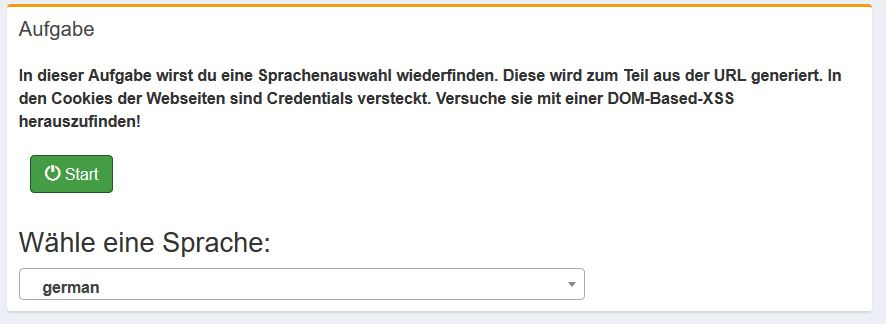
\includegraphics[width=\textwidth]{images/XSS/dom-based-xss-aufgabe.jpg}
	\caption{Aufgabenstellung des DOM-based-XSS Tutorials}
	\label{fig:dom-based-xss-aufgabe}
\end{figure}
Um das Tutorial zu lösen muss der Einsteiger die URL manipulieren, indem er dort ein Skript in die Anwendung injiziert. Hierzu soll der erneut die Cookies auslesen. Die Lösung für das Tutorial ist somit: 
\begin{center} 
\colorbox{altgray}{\lstinline|.../DOMbasedXSS.html?default=german<script>alert("document.cookie");</script>|} 
\end{center}
Abschließend muss hier erwähnt werden, dass auch dieses Tutorial ein Theorievideo sowie Tipps und Gegenmaßnahmen besitzt. 





